\section{2020 年 11 月 15 日答疑记录}

\begin{example}\label{exa:201204-1920}
    若 $a>b$, 且 $a-\dfrac1a> b-\dfrac1b$, 求 $ab$ 的取值范围.
\end{example}
\begin{solution}
    后一不等式变形为
    \[a-b-\frac1a+\frac1b>0,\quad\text{即}\quad
      a-b+\frac{a-b}{ab}>0.\]
    由 $a>b$ 知 $a-b>0$, 上式两边同时除以 $a-b$ 得
    \[1+\frac1{ab}>0,\quad\text{即 (通分后化为乘法)}\quad (1+ab)ab>0.\]
    将 $ab$ 视为整体, 解得 $ab\in(-\infty,-1)\cup (0,+\infty)$.
\end{solution}

\begin{example}\label{exa:201206-1410}
    若 $a$, $b>0$, 则 ``$a>b$'' 是 ``$a-\dfrac1a> b-\dfrac1b$'' 的什么条件?
\end{example}
\begin{solution}
    方法一: 由例~\ref{exa:201204-1920} 中的变形过程可知
    \[a-\dfrac1a> b-\dfrac1b\Rightarrow
        (a-b)\biggl(1+\frac1{ab}\biggr)>0.\]
    再由 $a$, $b>0$ 得 $ab>0$, 即 $1+\dfrac1{ab}>0$, 所以上式等价于 $a-b>0$. 这表明 ``$a>b$'' 是 ``$a-\dfrac1a> b-\dfrac1b$'' 的充要条件.
    
    方法二: 构造函数 $f(x)=x-\dfrac1x$ ($x>0$), 则不等式 $a-\dfrac1a> b-\dfrac1b$ 化为 $f(a)>f(b)$. 因为 $\dfrac1x$ 在 $(0,+\infty)$ 上单调递减, 所以 $-\dfrac1x$ 在 $(0,+\infty)$ 上单调递增. 而 $x$ 在 $(0,+\infty)$ 上也单调递增, 所以 $f(x)=x-\dfrac1x$ ($x>0$) 单调递增. 这表明 $f(a)>f(b)\Leftrightarrow a>b$, 所求为充要条件.
\end{solution}

{\bfseries 重要结论}(建议理解记忆)\quad 实际上 $f(x)=x-\dfrac1x$ ($x\neq0$) 在 $(-\infty,0)$ 和 $(0,+\infty)$ 上都是单调递增的, 其图形如下:

    \begin{center}
        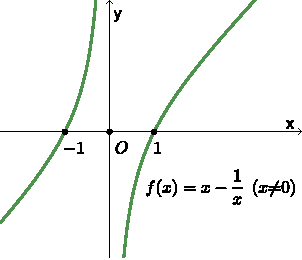
\includegraphics[scale=1]{2020-1204-1935-crop}
    \end{center}
    
\begin{example}
    判断函数 $y=|x+2|$ 在区间 $[-3,0]$ 上的单调性.
\end{example}
\begin{solution}
    方法一: 当 $x\in[-3,-2]$ 时, 
    \[y=|x+2|=\begin{cases}
        x+2, & -2\leqslant x\leqslant 0,\\
        -x-2, & -3\leqslant x<-2,
    \end{cases}\]
    由此可知, 该函数在 $[-3,-2)$ 上单调递减, 在 $[-2,0]$ 上单调递增.
    
    方法二: 直接作出 $y=|x+2|$ 的图形 (可先化为分段函数, 或参考 ``2020 年 9 月 26 日答疑记录'' 的第二部分), 单调性同上.
\end{solution}

\begin{example}
    设奇函数函数 $f(x)$ 在 $(-\infty,+\infty)$ 上单调递减, 且 $f(1)=-1$, 求不等式 $-1\leqslant f(x-1)\leqslant 1$ 的解集.
\end{example}
\begin{solution}
    因为 $f(x)$ 为奇函数, 所以由 $f(1)=-1$ 可知 $f(-1)=1$, 不等式化为
    \[f(1)\leqslant f(x-1)\leqslant f(-1).\]
    又因为 $f(x)$ 在 $(-\infty,+\infty)$ 上单调递减, 所以
    \[1\geqslant x-1\geqslant -1,\quad\text{解得}\quad 
        0\leqslant x\leqslant 2,\]
    即所求解集为 $[0,2]$.
\end{solution}

\begin{example}\label{exa:201204-2125}
    已知定义在 $\realnum$ 上的奇函数 $f(x)$ 满足 $f(x+4)=f(x)$ 且 $f(1)=1$, 求 $f(3)+f(4)+f(5)$ 的值.
\end{example}
\begin{solution}
    对定义在 $\realnum$ 上的奇函数 $f(x)$, 恒有 $f(-x)=-f(x)$. 令 $x=0$ 得 $f(0)=-f(0)$, 所以 $f(0)=0$. 结合 $f(x+4)=f(x)$ 知,
    \[\begin{aligned}
        \text{令 $x=0$:}&\ f(4)=f(0)=0,\\
        \text{令 $x=1$:}&\ f(5)=f(1)=1,\\
        \text{令 $x=-1$:}&\ f(3)=f(-1)=-f(1)=-1.
    \end{aligned}\]
    所以 $f(3)+f(4)+f(5)= (-1)+0+1=0$.
\end{solution}

\begin{remark}
    (1) 由上面的解法可知, 条件 ``$f(1)=1$'' 是多余的, 因为只需要推出 $f(4)=0$ 和 $f(3)=-f(1)$ 即可得到最终结论.
    
    (2) 例~\ref{exa:201204-2125} 中还证明了一个结论 (可当作定理直接使用): 若 $f(x)$ 为定义在 $\realnum$ 上的奇函数, 则 $f(0)=0$.
\end{remark}